\documentclass{article}
\usepackage[utf8]{inputenc}
\usepackage[spanish]{babel}
\usepackage{listings}
\usepackage{graphicx}
\graphicspath{ {images/} }
\usepackage{cite}

\begin{document}

\begin{titlepage}
    \begin{center}
        \vspace*{1cm}
            
        \Huge
        \textbf{Parcial 1}
            
        \vspace{0.5cm}
        \LARGE
        Desarrollo Parcial
            
        \vspace{1.5cm}
            
        \textbf{Sergio Giraldo Salazar y Ricardo Echeverri Cano}
            
        \vfill
            
        \vspace{0.8cm}
            
        \Large
        Departamento de Ingeniería Electrónica y Telecomunicaciones\\
        Universidad de Antioquia\\
        Medellín\\
        Marzo de 2021
            
    \end{center}
\end{titlepage}

\tableofcontents
\newpage
\section{Desarrollo del circuito}\label{Circuito}
Para resolver el trabajo pedido empezamos organizando el circuito el cual permitira dar solución a lo pedido y a su vez posibilitara que el software haga su función de manera correcta.

En esta primera parte buscamos con que resistencias se podia trabajar para que los leds pudieran encender al máximo.

\begin{figure}[h]
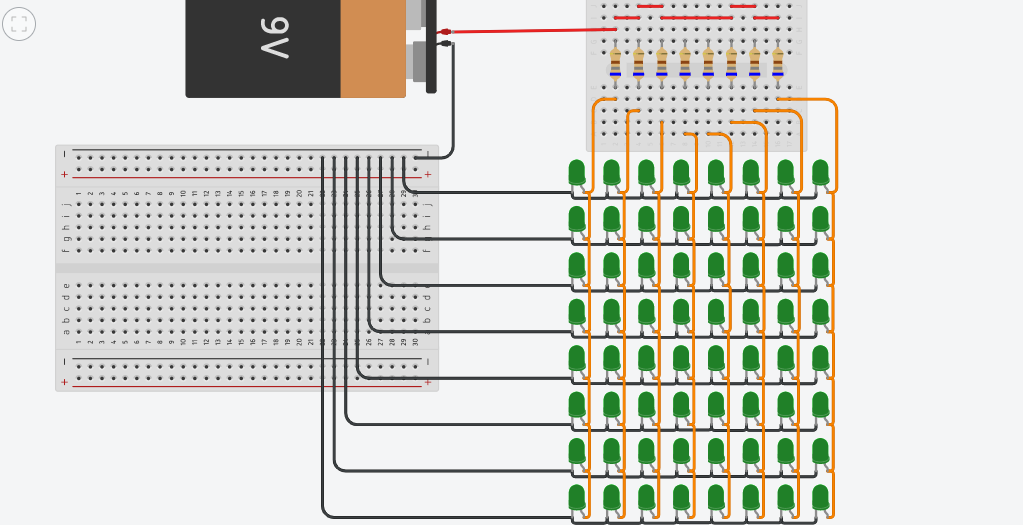
\includegraphics[width=10cm]{1.png}
\centering
\caption{Progreso 1}
\label{fig:primeros pasos}
\end{figure}
Luego organizamos los circuitos integrados conectandolos al arduino y también a la matriz de leds.

\begin{figure}[h]
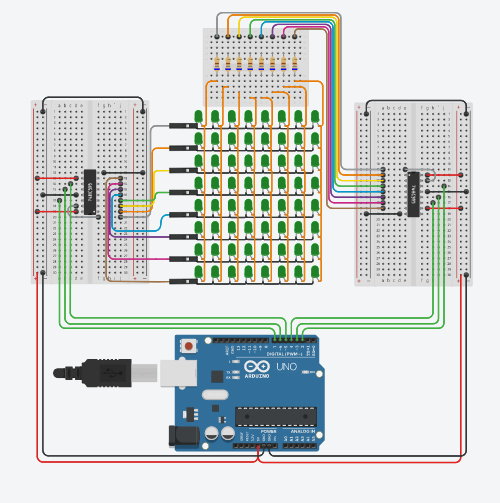
\includegraphics[width=10cm]{2.png}
\centering
\caption{Progreso 2}
\label{fig:primeros pasos}
\end{figure}

\end{document}